\section{Experimentos e resultados} 

Dado que o sistema de planejamento é geral, foram feitos dois experimentos, para o mundo dos blocos e para o mundo dos satélites. Os dados de entrada são os proporcionados na página no curso (ver \cite{LabIA15}).

\subsection{Experimentos com mundo dos blocos}
\label{subsec:expblocos}
	A figura~\ref{fig:blockssize} mostra os tamanhos do plano de solução do sistema de planejamento para problemas de 4 a 8 blocos e mostra que enquanto o número de blocos aumenta, o tamanho do plano não muda muito.
		\begin{figure}[H]
			\centering
			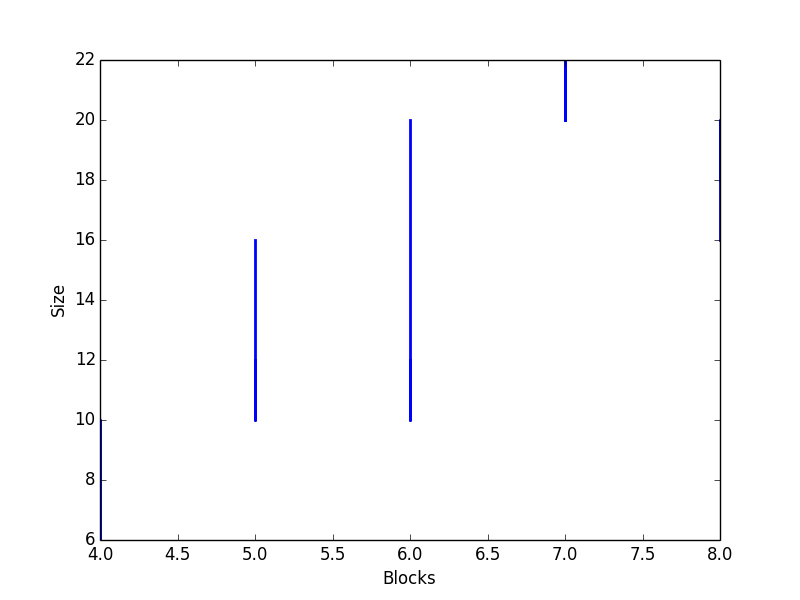
\includegraphics[height=8cm]{images/blocks-size}
			\caption{Tamanhos do plano de solução}
			\label{fig:blockssize}
		\end{figure}
	Mas na figura~\ref{fig:blockstime} se poder ver que os tempos de execução aumentam consideravelmente enquanto o número de blocos aumenta desde segundos até mais de uma hora para 8 blocos.
		\begin{figure}[H]
			\centering
			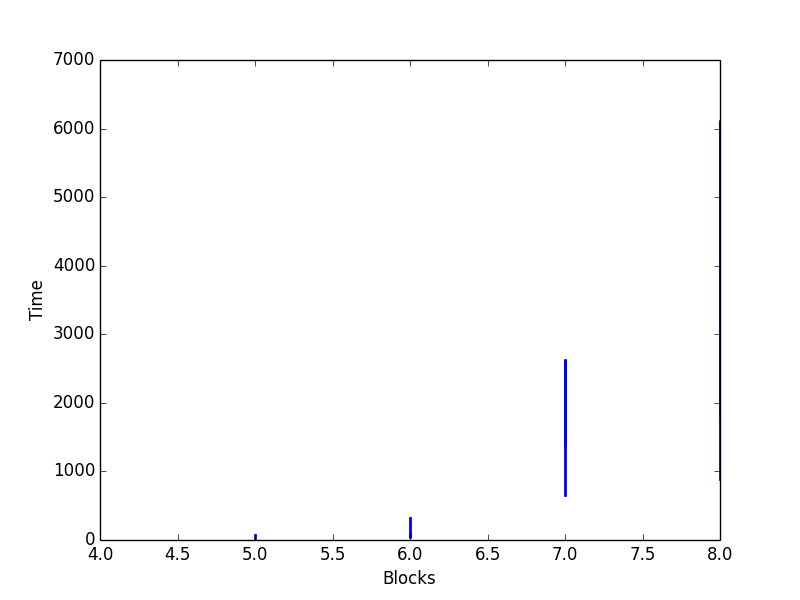
\includegraphics[height=8cm]{images/blocks-time}
			\caption{Tempo de execução (segundos)}
			\label{fig:blockstime}
		\end{figure}
	Além disso, o número de proposições necessárias para solucionar o problema sempre aumenta apesar que o tamanho do plano não muda muito.
		\begin{figure}[H]
			\centering
			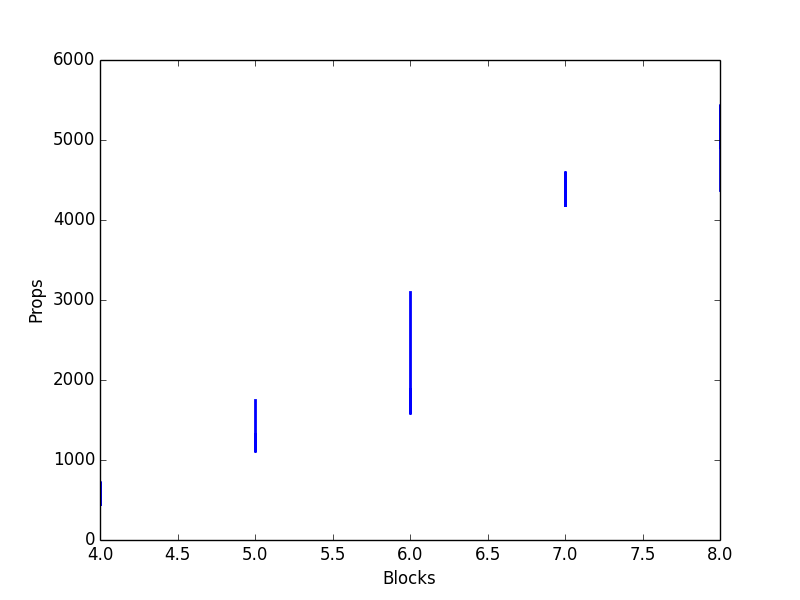
\includegraphics[height=8cm]{images/blocks-props}
			\caption{Número de proposições}
			\label{fig:blocksprops}
		\end{figure}
	Por último, o número de cláusulas aumenta exponencialmente devido que se tem mais variáveis e portanto mais valores para evaluar as ações e fluentes, o que também adiciona mais axiomas em cada iteração do algoritmo. 
		\begin{figure}[H]
			\centering
			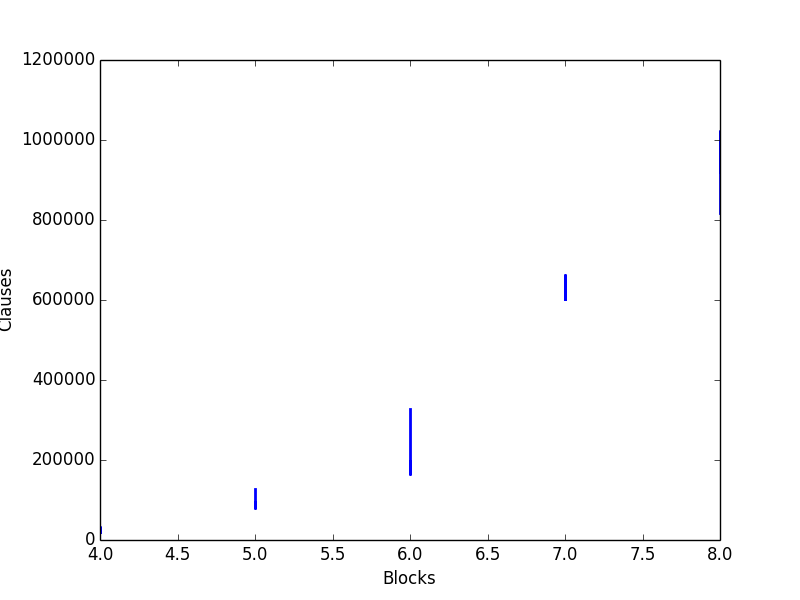
\includegraphics[height=8cm]{images/blocks-clauses}
			\caption{Número de cláusulas}
			\label{fig:blocksclauses}
		\end{figure}
		
 \subsection{Experimentos com mundo dos satelites}
\label{subsec:expsatelites}
	A figura~\ref{fig:satsize} mostra os tamanhos do plano de solução do sistema de planejamento para problemas de 1 a 5 satélites e mostra que enquanto o número de blocos aumenta, o tamanho do plano não muda muito.
		\begin{figure}[H]
			\centering
			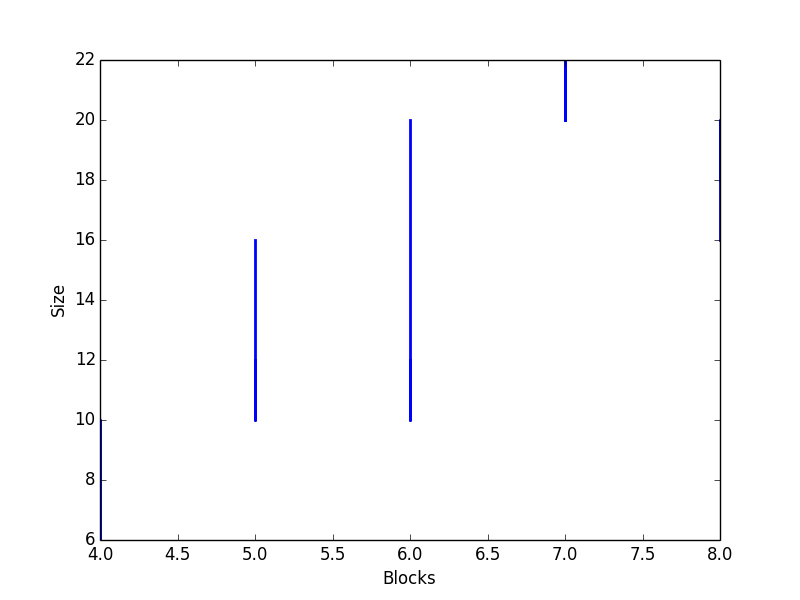
\includegraphics[height=8cm]{images/blocks-size}
			\caption{Tamanhos do plano de solução}
			\label{fig:satsize}
		\end{figure}
	Mas na figura~\ref{fig:sattime} se poder ver que os tempos de execução aumentam consideravelmente enquanto o número de blocos aumenta desde segundos até mais de uma hora para 8 blocos.
		\begin{figure}[H]
			\centering
			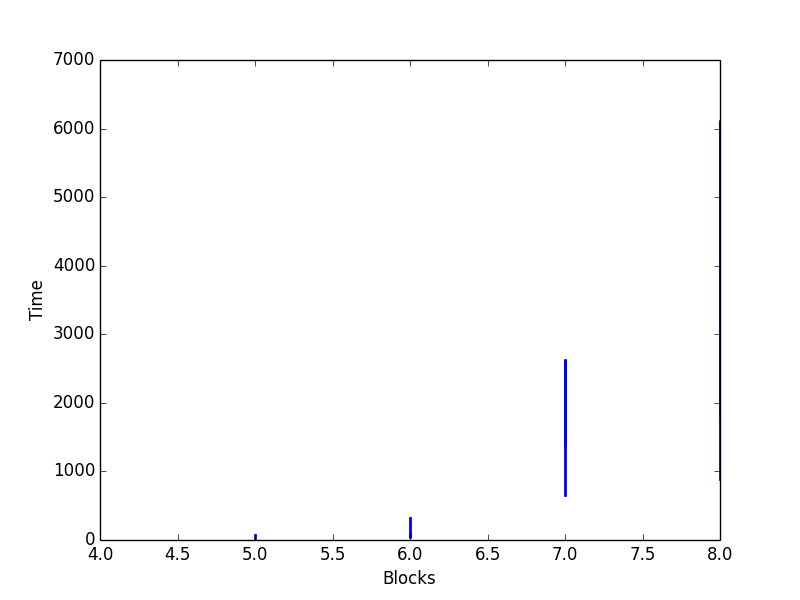
\includegraphics[height=8cm]{images/blocks-time}
			\caption{Tempo de execução (segundos)}
			\label{fig:sattime}
		\end{figure}
	Além disso, o número de proposições necessárias para solucionar o problema sempre aumenta apesar que o tamanho do plano não muda muito.
		\begin{figure}[H]
			\centering
			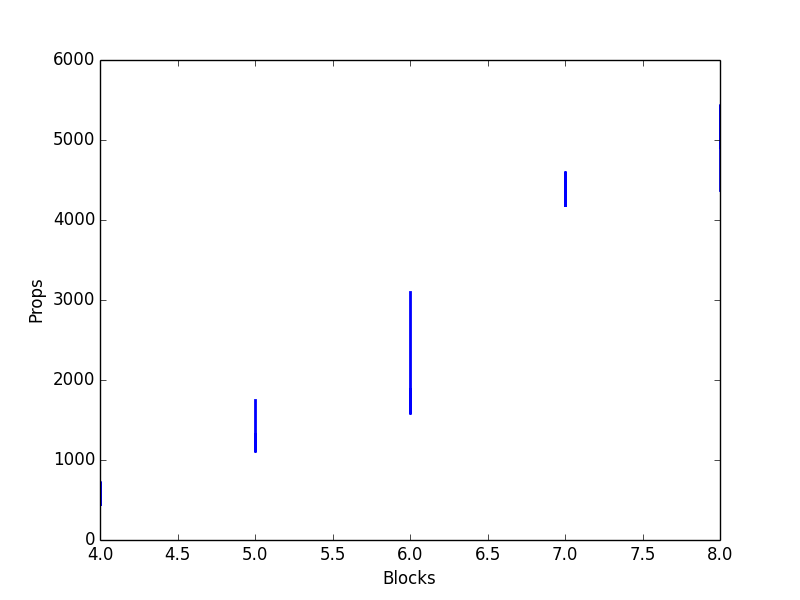
\includegraphics[height=8cm]{images/blocks-props}
			\caption{Número de proposições}
			\label{fig:satprops}
		\end{figure}
	Por último, o número de cláusulas aumenta exponencialmente devido que se tem mais variáveis e portanto mais valores para evaluar as ações e fluentes, o que também adiciona mais axiomas em cada iteração do algoritmo. 
		\begin{figure}[H]
			\centering
			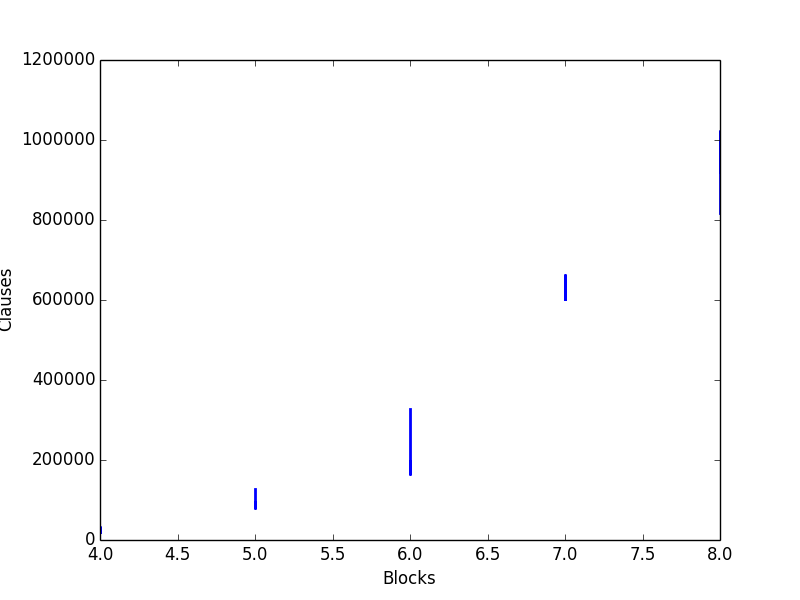
\includegraphics[height=8cm]{images/blocks-clauses}
			\caption{Número de cláusulas}
			\label{fig:satclauses}
		\end{figure}